\section{Statistics}\label{sec:statistics}

Every scientific investigation starts with a hypothesis that is to be tested empirically. The main objective is to evaluate if the proposed hypothesis agrees or disagrees with observed data, to either accept or reject it against the null-hypothesis. The metric at hand to do so is the p-value that arises within hypothesis testing. 

In the field of high-energy physics, a framework based on likelihood statistics has been developed specifically for this task. This section begins to lay out the mathematical fundamentals of the approach and explains its implementation in \textsc{pyhf}. The following is based on \citep{cowan2011asymptotic,behnke2013data,pyhf_intro}.

\subsection{Building the likelihood}
The statistical model must take into account how compatible the observed collision events are with the theoretical predictions. This can be described by a likelihood $L(\bm{x} | \bm{\phi})$ that is just a probability for an observation $\bm{x}$ under a given set of parameters $\bm{\phi}$. Since we are dealing with a counting experiment the tool at hand will be bins of a histogram $\bm{h}=(h_1,...,h_N)$. 

It is useful to subdivide a measurement $\bm{x}=(\bm{n},\bm{a})$ further into a quantity of interest $\bm{n}$, (e.g. the invariant mass of a particle) and \textit{auxiliary} measurement histograms $\bm{a}$ that help to constrain the model. Additionally in the context of hypothesis testing it is useful to split the set of parameters $\bm{\phi}=(\bm{\psi},\bm{\Theta})$ into so called parameters of interest $\bm{\psi}$ and nuisance parameters $\bm{\Theta}$. For this section the parameter of interest will be only one parameter, the signal strength $\mu$. 

The bin heights (counts) can then be expressed in terms of the amount of signal $s_i(\bm{\Theta})$ and background $b_i(\bm{\Theta})$ in them depending in some way on the nuisance parameters. The prediction (expectation value) of the $n_i$ can then be expressed as
\begin{equation} \label{eq:n_i}
    \langle n_i(\mu,\bm{\Theta})\rangle = \mu s_i(\bm{\Theta}) +b_i(\bm{\Theta}), 
\end{equation}
and similar for the $a_i$
\begin{equation} \label{eq:a_i}
    \langle a_i(\bm{\Theta}) \rangle = u_i(\bm{\Theta}).
\end{equation}
As we are expecting the bin counts to occur with a constant mean rate and independent of time compared to the last event, each bin follows a Poisson distribution
\begin{equation}\label{eq:poisson}
    \frac{r^k e^{-r}}{k!}.
\end{equation}
$r$ is the expected rate of occurrences, which translates as our prediction, whereas $k$ are the actual measured occurrences. Accounting for all the bins $N$ by multiplying them together yields
\begin{equation}\label{eq:likelihood}
    L(\mu,\bm{\Theta})=
    \prod_{j=1}^N \frac{(\mu s_j(\bm{\Theta}) + b_j(\bm{\Theta}))^{n_j}}{n_j !} e^{-(\mu s_j(\bm{\Theta}) + b_j(\bm{\Theta}))}
    \prod_{k=1}^M \frac{u_k(\bm{\Theta})^{a_k}}{a_k!} e^{-u_k(\bm{\Theta})}.
\end{equation}
The last product can also be thought of penalizing the likelihood if e.g. an auxiliary measurement displays a very improbable value for a quantity. To test for a hypothesized value of $\mu$, the best choice according to the Neyman-Pearson lemma, is the profile likelihood ratio that reduces the dependence to the parameter(s) of interest
\begin{equation}
\lambda(\mu)=
    \frac{L(\mu,\hat{\hat{\bm{\Theta}}})}
    {L(\hat{\mu},\hat{\bm{\Theta}})}
\end{equation}
The denominator is the unconditional maximum likelihood estimation so that $\hat{\mu}$ and $\hat{\bm{\Theta}}$ both are free to vary to maximize $L$, whereas the numerator is the found maximum likelihood conditioned on some chosen $\mu$ and the set nuisance parameters $\hat{\hat{\bm{\Theta}}}$ that maximize the likelihood for that particular $\mu$. This definition gives $0 \leq \lambda \leq 1$. For a $\lambda \approx 1$ the hypothesized value of $\mu$ shows good agreement to the Poissonian model.

\subsection{From test statistic to p-value}   
Transforming the profile likelihood into a test statistic $t_{\mu}$ is practical to calculate p-values
\begin{equation}
    t_{\mu}=-2\log \lambda(\mu).
\end{equation}
This translates as $t_{\mu} \rightarrow 0$ as good agreement, $t_{\mu} \rightarrow \infty$ as bad agreement to the model. A right-tail p-value can then be calculated from the probability density function of $t_\mu$: pdf$(t_\mu) = f(t_\mu \mid \mu)$
\begin{equation}\label{eq:p-value}
    p_\mu = \int_{t_{\mu ,obs}}^{\infty} 
    f(t_\mu \mid \mu) \mathrm{d}t_\mu
\end{equation}
$t_{\mu ,obs}$ is the test statistic $t_\mu$ evaluated at the observed data. This is like plugging into the Poisson distributions the same values for $r$ as for $k$ in eq. \ref{eq:poisson}. Just like a probability density function for a standard normal distribution, intuitively the pdf is just, how probable a particular value of the test statistic $t_\mu$ is under a fixed value of the signal strength (how often it occurs compared to all other values $t_\mu$ can have). 

This particular form is handy because there exist approximations for $f(t_\mu \mid \mu)$ \citep{cowan2011asymptotic}. Wald \citep{wald1943tests} proved that in the large sample limit the test statistic follows a normalized sum of squared distances between the tested parameter of interest $\mu_i$ and its maximum likelihood estimate $\hat{\mu}_i$. The result was extended by Wilk \citep{wilks1938large} for any number of parameters of interest so the test statistic becomes
\begin{equation}
    t_\mu=\sum_i \frac{(\mu_i-\hat{\mu}_i^2)}{\sigma_i^2} + \mathcal{O}(1/\sqrt{N}).
\end{equation}
The $\hat{\mu}_i$ are in the large sample limit normally distributed with mean $\mu'$ (true values) and standard deviation $\sigma_i$. This is the definition of a non-central chi-squared distribution with degrees of freedom $i$ equal to the parameters of interest (see section 3.1 in \citep{cowan2011asymptotic}). For one parameter of interest the distribution reads
\begin{equation}\label{eq:chi-square}
    f(t_\mu \mid \mu)=\frac{1}{2\sqrt{t_\mu}}\frac{1}{\sqrt{2\pi}}
    \left[
\exp\left(-\frac{1}{2}\left(\sqrt{t_\mu}+\sqrt{\Lambda}_\mu\right)\right)
+
\exp\left(-\frac{1}{2}\left(\sqrt{t_\mu}-\sqrt{\Lambda}_\mu\right)\right)
\right],
\end{equation}
with non-centrality parameter 
\begin{equation}
    \Lambda_\mu=\frac{(\mu-\mu')^2}{\sigma^2}.
\end{equation}
Figure \ref{fig:test_stat_example} illustrates the different steps. Being able to calculate p-values allows now to state how likely it is that the proposed hypothesis is reflected by the observed data. Put differently, if the experiment would be repeated the p-value represents the probability of that the outcome favors the alternative hypothesis over the null hypothesis.

In the scientific community a widely accepted threshold for this is a p-value of 0.05. Though particle physicists only claim discovery of a new phenomenon for $p$ < \SI{2.87e-7}{} (5 standard deviations of the standard normal distribution). One caveat here is that this particular form of $t_\mu$ assumes $\mu$ can also be negative, which can be non-physical depending on the impact of a new process. Test statistics and their pdf approximations considering the different cases are covered in \citep{cowan2011asymptotic}. 
\begin{figure}
    \centering
    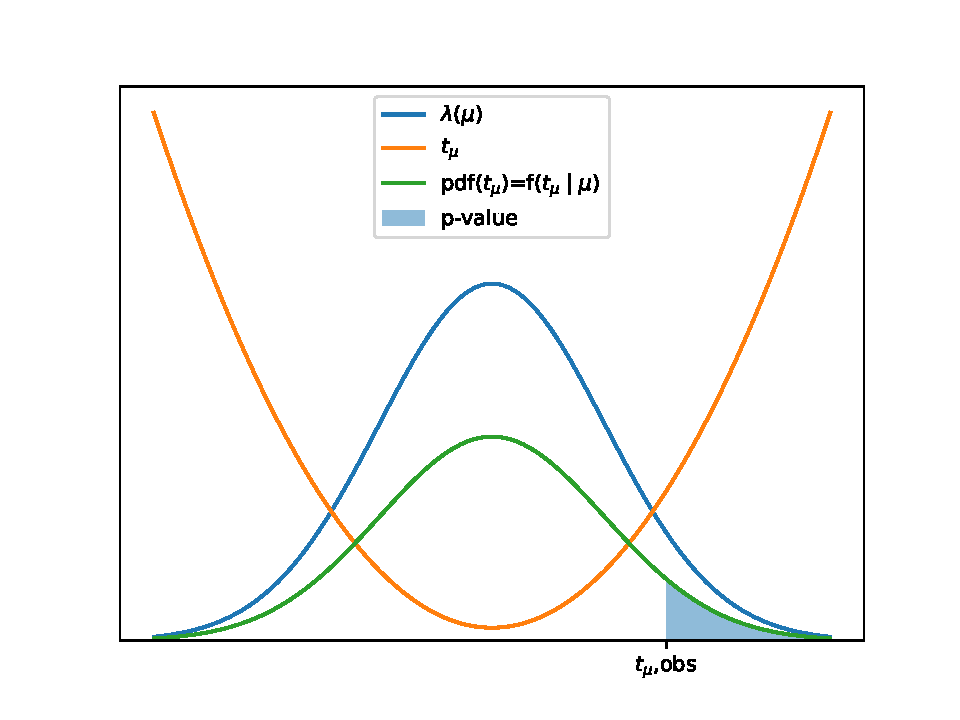
\includegraphics[width=0.8\textwidth]{test_stat_example.pdf}
        \caption[]{A sketch to follow the steps to calculate p-values. (\textbf{left}) The profile likelihood (\hexbox{1f77b4}) has essentially some hill-like form with a maximum at ${\lambda(\hat{\mu},\hat{\bm{\Theta}})}$, $t_\mu$ (\hexbox{ff7f0e}) is $-2\mathrm{ln}(\lambda)$. (\textbf{right}) For one parameter of interest in the large sample limit $f(t_\mu \mid \mu)$ follows a non-central chi-squared distribution with one degree of freedom, equation \ref{eq:chi-square}. The blue shaded area under the pdf is a right hand sided p-value.}
    \label{fig:test_stat_example}    
\end{figure}

\subsection{The CL$_s$ value}\label{sec:cls}

Particle physicists are usually interested in two things when making statistical tests for discovery of new phenomena: how well is the modeling of backgrounds (things we know) and if there is evidence in the observations for a new phenomenon. This means one needs to test two hypotheses: a background only ($b$) and a signal plus background ($s+b$) hypothesis. Each will result in a p-value on their own. For example $p_{b}=0$ would mean that the backgrounds are perfectly reflected by the observations and a $p_{s+b} < 0.05$ could be a sign of e.g. new physics. To combine these two metrics into a single score, particle physicists came up with the pseudo Confidence Level/p-value called CL$_s$ incorporating also the goodness of the modeling of the backgrounds 
\begin{equation}
    \mathrm{CL}_s=\frac{p_{s+b}}{1-p_{b}}=
    \frac
    {\int_{t_{\mu ,obs}}^{\infty} 
    f(t_\mu \mid \mu) \mathrm{d}t_\mu}
    {1-\int_{t_{\mu ,obs}}^{\infty} 
    f(t_\mu \mid \mu) \mathrm{d}t_\mu}.
\end{equation}
Intuitively the numerator is again just the value for the alternative hypothesis whereas the denominator penalizes CL$_s$ if the modeling of the backgrounds is not reflected in the observations. This can also be understood visually from the first figure of the heavily cited CL$_s$ paper that introduced the quantity \citep{read2002presentation} (see description of fig. \ref{fig:cls}).
\begin{figure}[H]
    \centering
    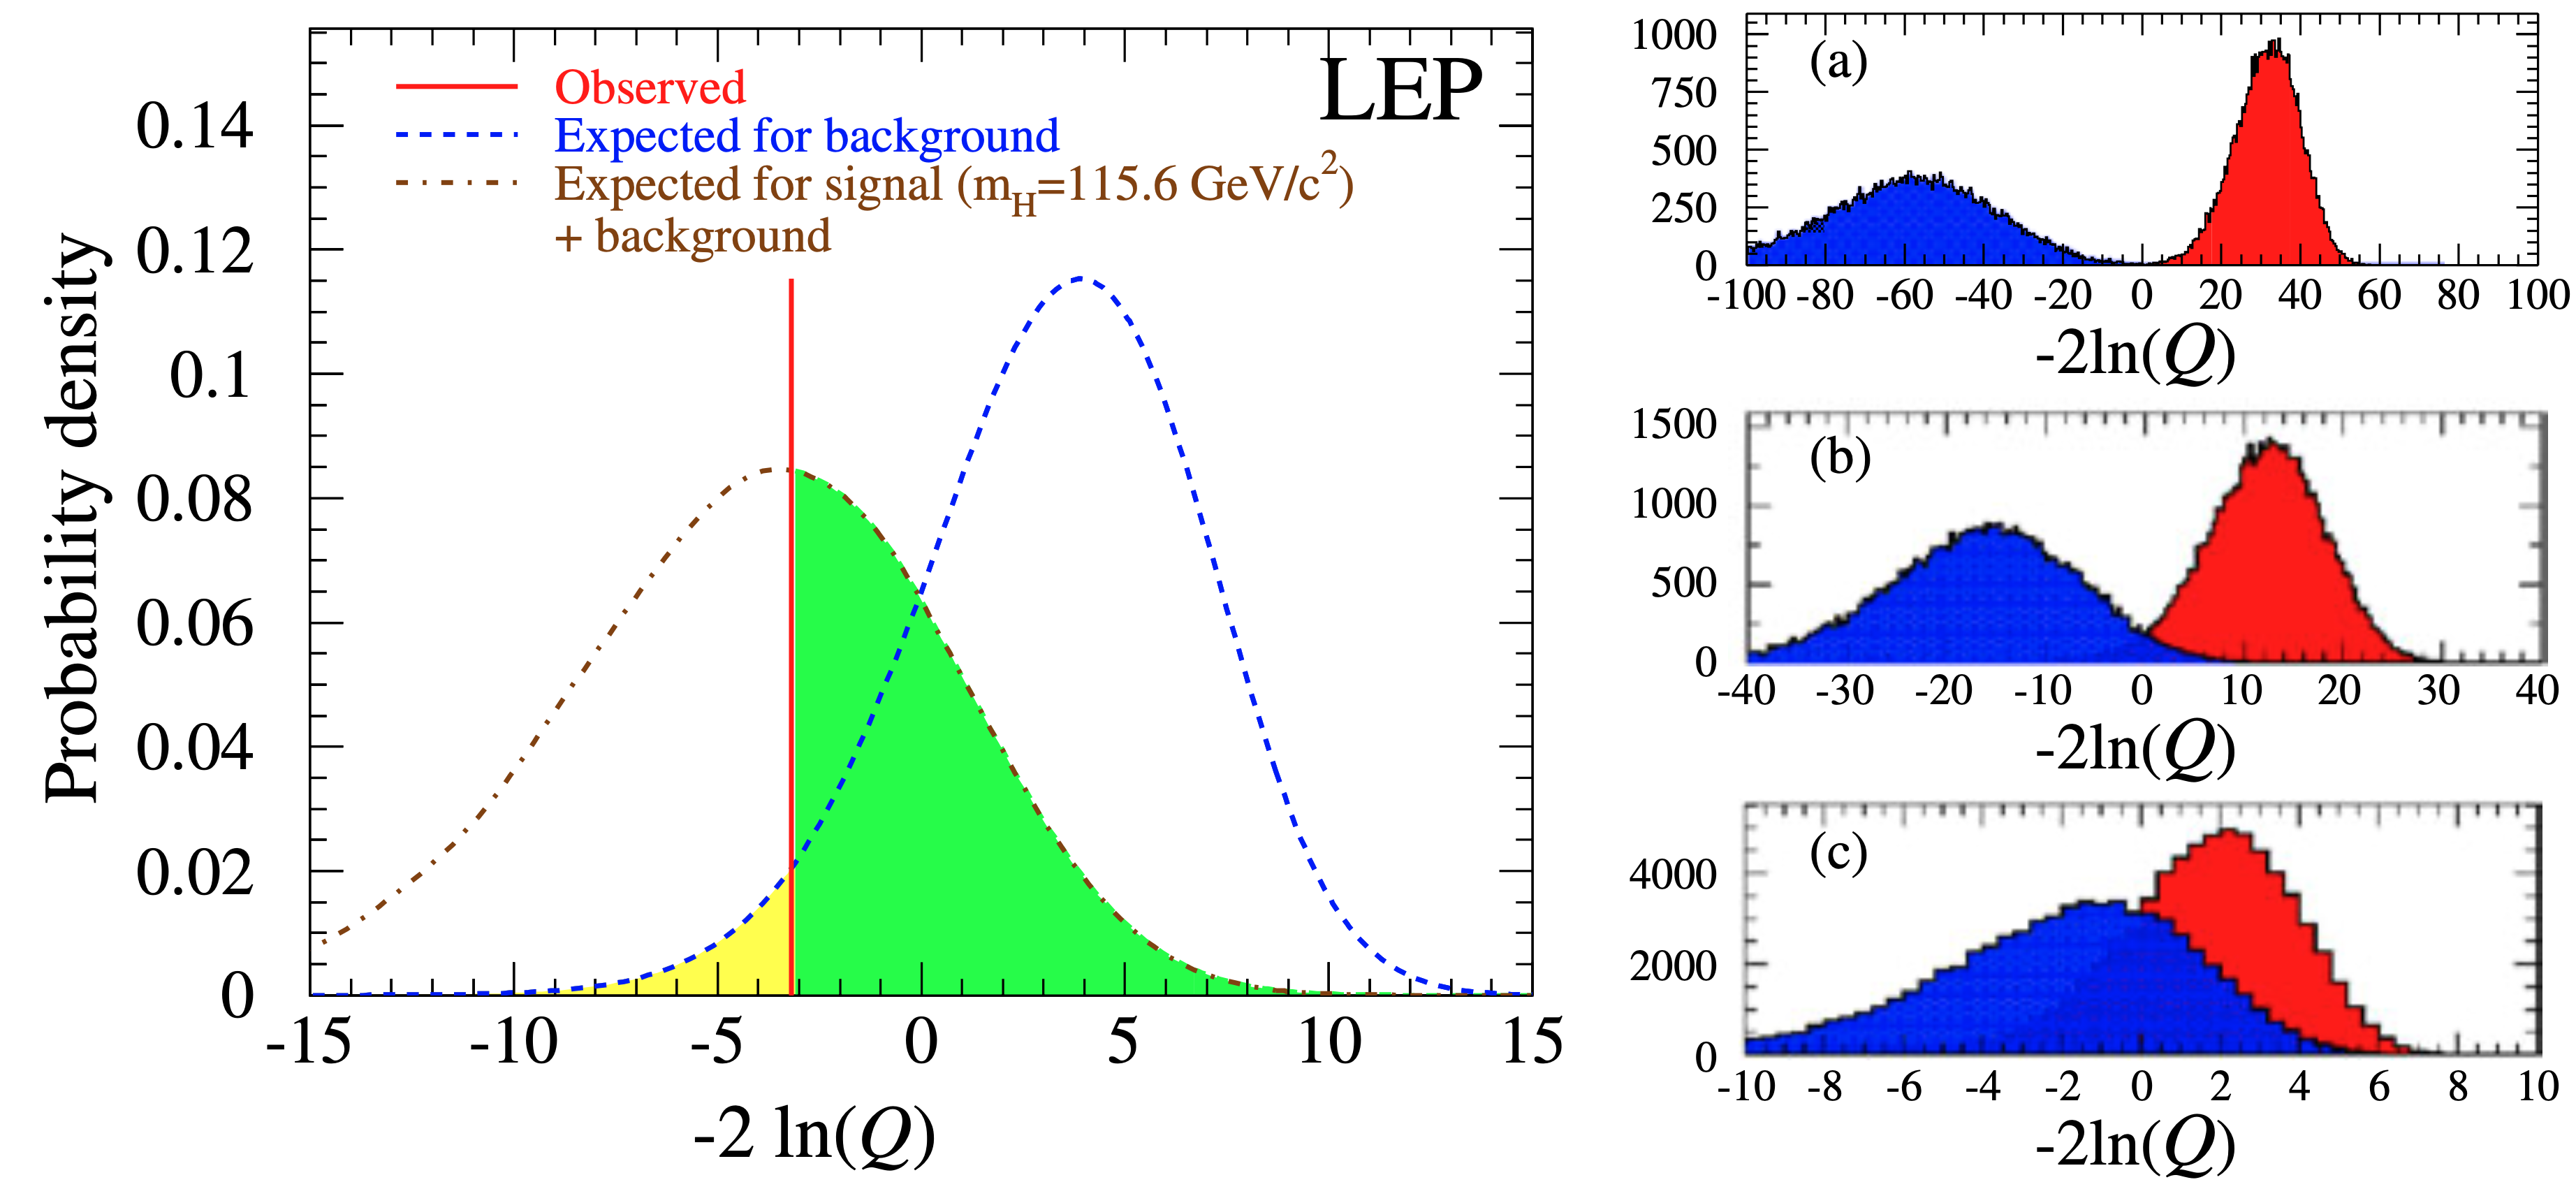
\includegraphics[width=1\textwidth]{cls.png}
        \caption[]{Probability density functions of test statistics from a Higgs search at LEP illustrating the calculation of p-values ($\lambda$ becomes $Q$). (\textbf{left}) The pdf's of the test statistic $f(t_\mu \mid \mu)$ of the signal + background ({\color[HTML]{804000}{$\diagup$}}) and background ({\color[HTML]{2100FF}{$\diagup$}}) only hypotheses. The p-value is calculated by integration from $t_{\mu,obs}$ (the red observed line ({\color[HTML]{FF0000}{$\diagup$}})) to infinity (see eq. \ref{eq:p-value}). The green shaded area (\hexbox{00FF00}) corresponds to $p_{s+b}$ whereas the yellow area (\hexbox{FDFF02}) corresponds to $1-p_b$ since the integral over one whole pdf is 1. (\textbf{right}) Degradation of search sensitivity from (a) to (c). Note that the colors of the pdf's change here to signal + background (\hexbox{2100FF}) and background only (\hexbox{FF0000}). For example putting the observation ($t_{\mu,obs}$) on the x-axis at 0 in these plots, one would get for plot (a) $p_{b}\approx 1$ and $p_{s+b}\approx 0$ resulting in a CL$_s\approx 0$, whereas with increasing overlap the CL$_s$ value increases and the sensitivity decreases.
        From \citep{read2002presentation}.}
    \label{fig:cls}    
\end{figure}



\subsection{The HistFactory model}

A model used widely to achieve the preceding for a typical ATLAS analysis is called HistFactory \citep{cranmer2012histfactory} and is implemented within \textsc{pyhf} \citep{heinrich2021pyhf}. This follows closely the introduction to the model within the documenation of \textsc{pyhf} \citep{pyhf_intro}. HistFactory draws the name from the idea that the problem is reducible to a small number of basic components. In order to build a likelihood like eq. \ref{eq:likelihood} it is again useful to think of another splitting of the nuisance parameters $\bm{\phi}$ into

\newcommand{\freeset}{\bm{\eta}}
\newcommand{\constrset}{\bm{\chi}}
\newcommand{\singleconstr}{\chi}
\newcommand{\channelcounts}{\bm{n}}
\newcommand{\auxdata}{\bm{a}}
\newcommand{\poiset}{\bm{\psi}}
\newcommand{\nuisset}{\bm{\theta}}
\newcommand{\fullset}{\bm{\phi}}
\newcommand{\singlefull}{\phi}


\begin{equation}
 L(\bm{x}|\fullset) \quad=\quad
 L(\bm{x}|\overbrace{\poiset}^{\llap{\text{parameters of interest}}},\underbrace{\nuisset}_{\llap{\text{nuisance parameters}}}) \quad=\quad
 L(\bm{x}|\overbrace{\freeset}^{\rlap{\text{free}}},\underbrace{\constrset}_{\rlap{\text{constrained}}}) 
\end{equation}
free parameters $\freeset$, for example a cross section of a process and constrained parameters $\constrset$, that incorporate systematic uncertainties. The likelihood can then be modeled with Poissonians for each of the channels $c$ (e.g. signal regions), bins $b$ and constraint terms $c_{\singleconstr}$ that again penalize the likelihood
\begin{equation}
L(\channelcounts, \auxdata \,|\,\freeset,\constrset) = \underbrace{\color{blue}{\prod_{c\in\mathrm{\,channels}} \prod_{b \in \mathrm{\,bins}_c}\textrm{Pois}\left(n_{cb} \,\middle|\, \nu_{cb}\left(\freeset,\constrset\right)\right)}}_{\substack{\text{Simultaneous measurement}\\%
\text{of multiple channels}}} \underbrace{\color{red}{\prod_{\singleconstr \in \constrset} c_{\singleconstr}(a_{\singleconstr} |\, \singleconstr)}}_{\substack{\text{constraint terms}\\%
\text{for }\text{auxiliary measurements}}}.
\end{equation}
The $n_{cb}$ is the observation and $\nu_{cb}(\freeset,\constrset)$ the prediction. The $c_{\singleconstr}$ are calculated from auxiliary measurements $a_{\singleconstr}$ to constrain $\singleconstr$ and can be any function (e.g. Gaussian, Poissonian,...) we believe the parameter to be distributed. 

The prediction is a sum of nominal bin height estimates $\nu_{scb}^0$ over all samples $s$ (e.g. $t\overline{t}$, multijet-background etc.). These nominal bin height estimates can be modified within associated errors. This enters the likelihood through the constraint terms $c_{\singleconstr}$ and multiplicative $\kappa_{scb}$ and additive modifiers $\Delta_{scb}$
\begin{align}
    \nu_{cb}\left(\fullset\right) &= \sum_{s\in\mathrm{\,samples}} \nu_{scb}\left(\freeset,\constrset\right)\\ &= \sum_{s\in\mathrm{\,samples}}\underbrace{\left(\prod_{\kappa\in\,\bm{\kappa}} \kappa_{scb}\left(\freeset,\constrset\right)\right)}_{\text{multiplicative modifiers}}\, \Bigg(\nu_{scb}^0\left(\freeset, \constrset\right) + \underbrace{\sum_{\Delta\in\bm{\Delta}} \Delta_{scb}\left(\freeset,\constrset\right)}_{\text{additive modifiers}}\Bigg).
\end{align}
To understand this approach let us consider one systematic. If we would modify the nominal bin height estimate $\nu_{scb}^0$ by some factor (modifier) while the penalization stays small (constraint term), it can be beneficial for our goal of maximizing the likelihood. This means we find the most likely/compatible value to the observed data within our modeling of the errors. 

In HistFactory there are by convention four types $\{ \gamma,\alpha,\lambda,\mu \}$ of such multiplicative rate modifiers that will be explained throughout the rest of this section. 

There are free rate modifiers $\lambda$ and $\mu$ that affect all bins equally, like the cross section of a process or the luminosity 
\begin{equation}
    \nu_{scb}(\mu)=\mu \nu_{scb}^0.
\end{equation}
These are bin-independent and shape(of the histogram)-preserving normalization factors and could be for example the signal strength from above.

In addition $\gamma_b$ denotes bin-wise parameters (uncorrelated shape)
\begin{equation}
    \nu_{scb}(\gamma_b)=\gamma_b \nu_{scb}^0.
\end{equation}
These are useful for example to include the Monte Karlo uncertainties or a per bin data-driven background estimate. This type without a constraint term has to be used with care as if there is only one sample or channel, the fit would always match the data perfectly, which of course is not of much use.

Further there are bin-independent (shape factors) nuisance parameters $\alpha$ that enter the modeling through an interpolation function $\eta$ instead of being the factor itself. There is the multiplicative version 
\begin{equation}
    \nu_{scb}(\alpha)=\eta(\alpha) \nu_{scb}^0,
\end{equation}
and the additive version
\begin{equation}
    \nu_{scb}(\alpha)=\nu_{scb}^0 + \eta(\alpha), 
\end{equation}
with some constraint term $c_\alpha(\alpha)$. This is useful if systematic uncertainties are to be included. In an ATLAS analysis typically this is done by plugging in the upper (`1up') and lower (`1down') standard deviation values (pretending they were the nominal values entering the calculation) and observe the impact it has on a final quantity. The interpolation function transports this knowledge into the likelihood model, by scaling the nominal value $\nu_{scb}^0$ and at the same time applying a penalization $c_\alpha$ according to our modeling of the errors. The following illustrates this.

In HistFactory there exists four of such interpolation functions. For those exist an identity operator 
\begin{equation}
    \eta_0=\eta (\alpha=0) =
    \begin{cases}
        1 ,& \text{multiplicative modifier, } (\kappa) \\
        0 ,& \text{additive modifier, } (\lambda).
    \end{cases}
\end{equation}
One of these interpolation function that scales the bin height linear over the known deviations $\eta_{-1}=\nu_{scb}^\mathrm{1down}$ and $\eta_{1}=\nu_{scb}^\mathrm{1up}$ is
\begin{equation}
    \eta_\mathrm{linear}(\alpha)=
    \begin{cases}
        \alpha(\eta_0 - \eta_1) ,& \alpha>0\\
        \alpha(\eta_0 - \eta_{-1}) ,& \alpha<0
    \end{cases}
\end{equation}
An illustration of this can be found in fig. \ref{fig:interp_func}(a). For the other ones the reader is referred to e.g. \citep{heinrich2019searches}. 
\begin{figure}
    \centering
    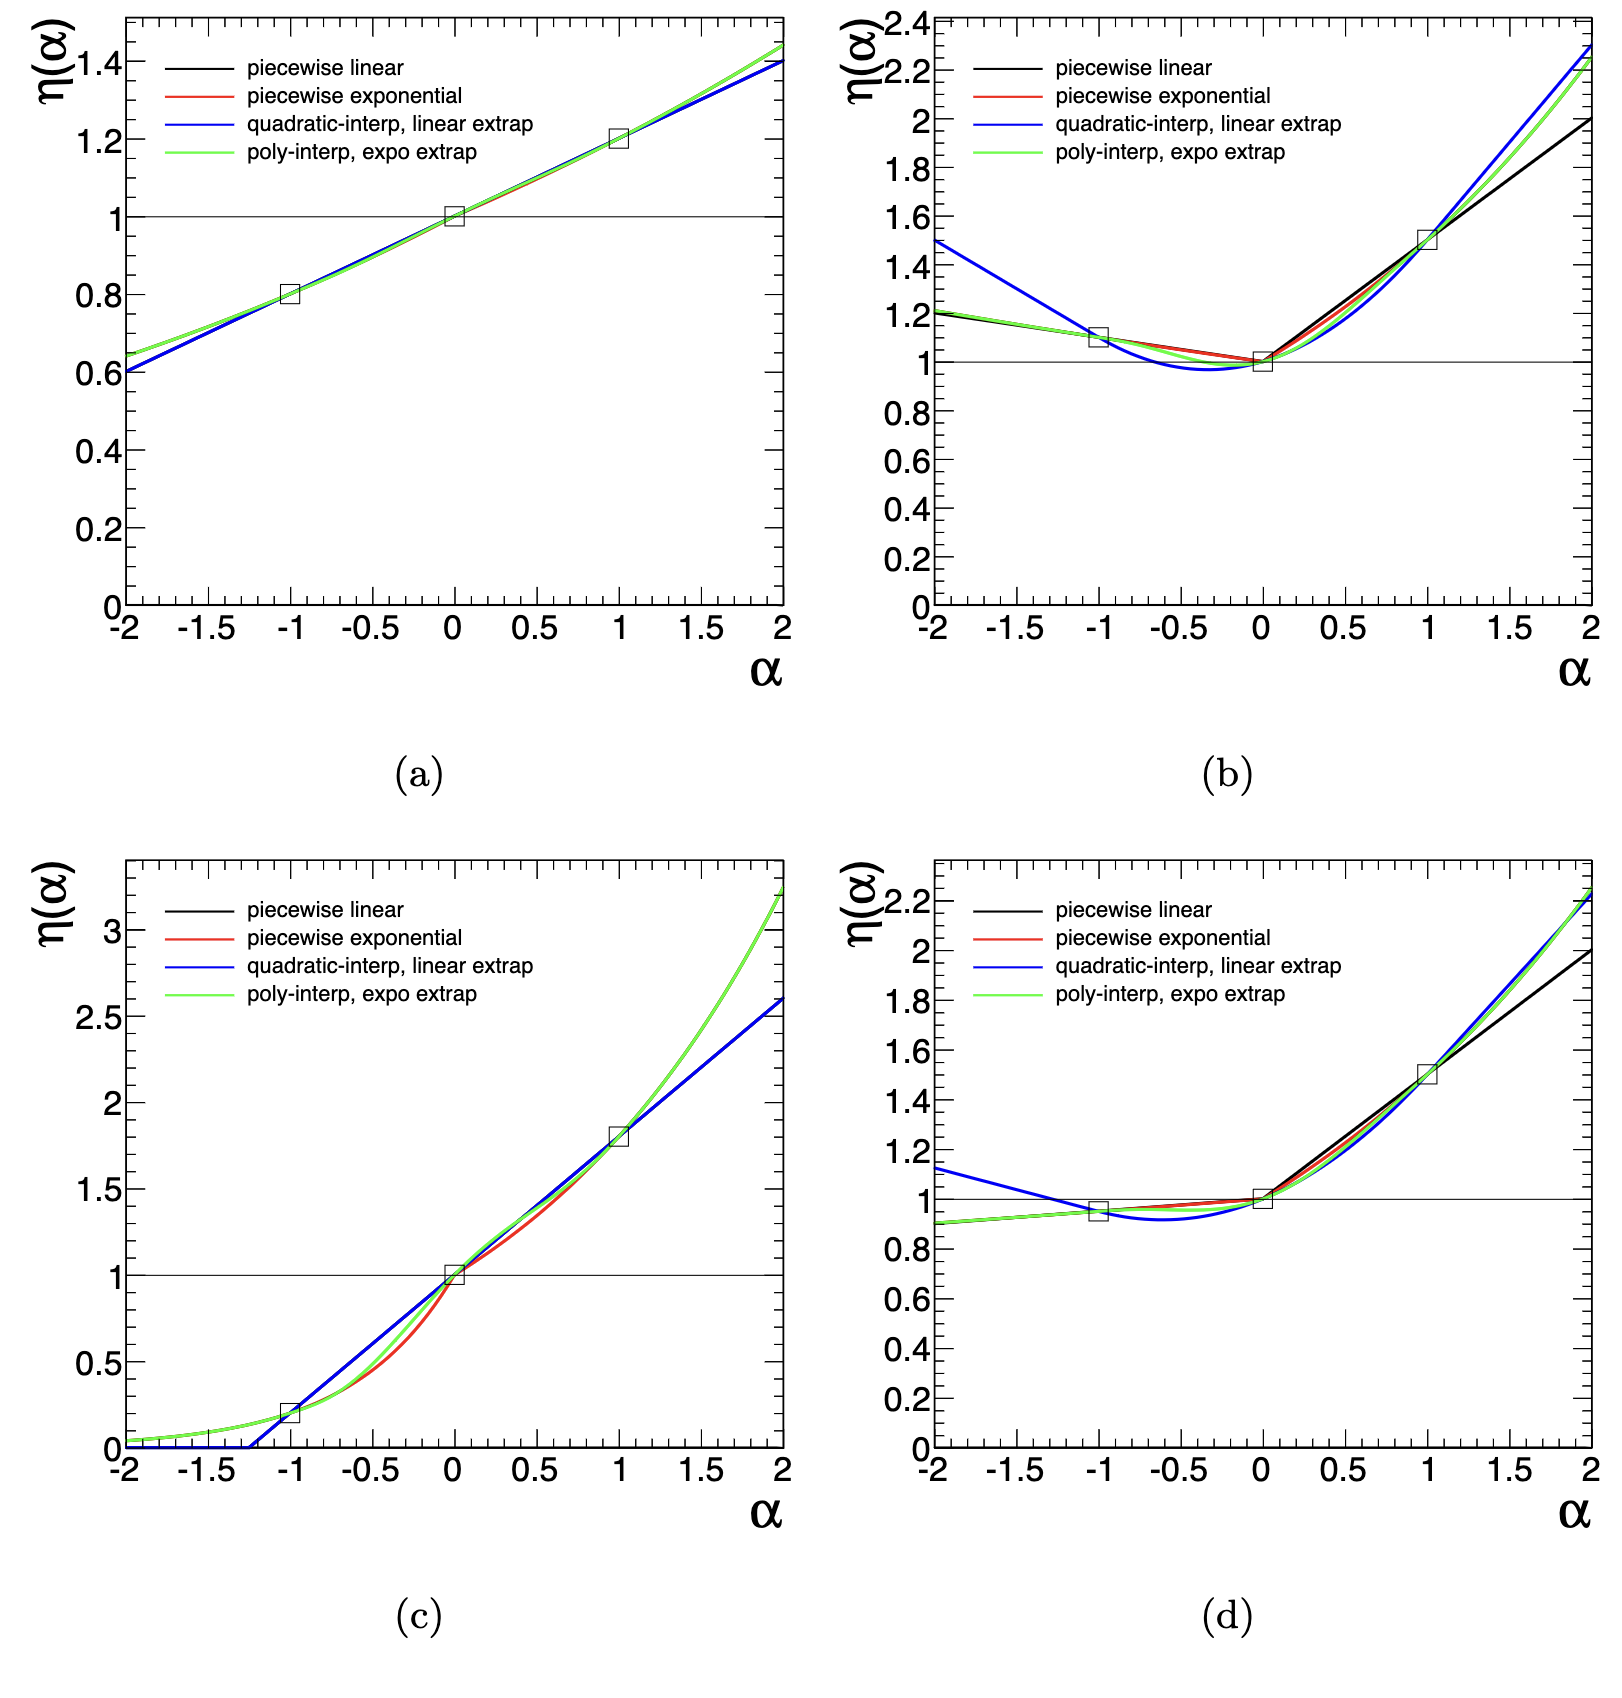
\includegraphics[width=.8\textwidth]{interp_func.png}
        \caption[]{The four Interpolation functions $\eta(\alpha)$ for different up and down standard deviation values. For example in (a) the bin height will be scaled with a factor of 0.8 for an $\alpha=-1$ (1.2 for an $\alpha=1$). From \citep{cranmer2012histfactory}.}
    \label{fig:interp_func}    
\end{figure}
Remember $\alpha$ is the nuisance parameter and not the function $\eta(\alpha)$ and there is an associated constraint term $c_\alpha$ to each $\alpha$ that uses Gaussian and Poissonian modeling. The standard normal Gaussian  implementation is straightforward as the nuisance parameter is scaled to the standard deviation values as described before Gauss$=(\alpha \mid a, \sigma=1)$. 

For a poissonian constraint to a multiplicative factor $\gamma_b$, with a nominal (most probable) value $\gamma_0=1$, we must scale the Poisson distribution with a factor $f$ so it reflects the original bin-height uncertainty $\sigma$. We basically need to multiply all parameters of the Poisson distribution with a factor f and then solve for the one with the desired uncertainty. Since the Variance of a Poissonian like eq. \ref{eq:poisson} is just the rate parameter $\lambda$ it follows
\begin{equation}
    \mathrm{Var}(\mathrm{Pois}(k=f\gamma_0,\lambda=f\gamma))=\lambda\stackrel{\gamma=\gamma_0}{=}f\gamma_0=(f\sigma)^2  \quad \rightarrow \quad f=(1/\sigma^2).
\end{equation}
This completes all the requirements needed for the creation of histfactory models. The different types of modifiers and their constraint terms are summarized in table \ref{tab:histfactory}.
\begin{table}[]
    \caption[]{Modifiers and constraint terms used in HistFactory implemented by pyhf. Note that the interpolation functions are called $f_p$ and $g_p$ here instead of $\eta$ as chosen in the full text.  From \citep{pyhf_intro}}
    \centering
    \resizebox{0.97\textwidth}{!}{
        \begin{tabular}{l|l|l|l}\label{tab:histfactory}
            Description &Modification&Constraint Term $c_\singleconstr$ &$c_\chi$ input\\
            \hline
            Uncorrelated Shape   &$\kappa_{scb}(\gamma_b) = \gamma_b$                                                                     &$\prod_b \mathrm{Pois}\left(r_b = \sigma_b^{-2}\middle|\,\rho_b = \sigma_b^{-2}\gamma_b\right)$ &$\sigma_{b}$    \\
            Correlated Shape     &$\Delta_{scb}(\alpha) = f_p\left(\alpha\middle|\,\Delta_{scb,\alpha=-1},\Delta_{scb,\alpha = 1}\right)$ &$\displaystyle\mathrm{Gaus}\left(a = 0\middle|\,\alpha,\sigma = 1\right)$                       &$\Delta_{scb,\alpha=\pm1}$    \\
            Normalisation Unc.   &$\kappa_{scb}(\alpha) = g_p\left(\alpha\middle|\,\kappa_{scb,\alpha=-1},\kappa_{scb,\alpha=1}\right)$   &$\displaystyle\mathrm{Gaus}\left(a = 0\middle|\,\alpha,\sigma = 1\right)$                       &$\kappa_{scb,\alpha=\pm1}$    \\
            MC Stat. Uncertainty &$\kappa_{scb}(\gamma_b) = \gamma_b$                                                                     &$\prod_b \mathrm{Gaus}\left(a_{\gamma_b} = 1\middle|\,\gamma_b,\delta_b\right)$                 &$\delta_b^2 = \sum_s\delta^2_{sb}$    \\
            Luminosity           &$\kappa_{scb}(\lambda) = \lambda$                                                                       &$\displaystyle\mathrm{Gaus}\left(l = \lambda_0\middle|\,\lambda,\sigma_\lambda\right)$          &$\lambda_0,\sigma_\lambda$    \\
            Normalisation        &$\kappa_{scb}(\mu_b) = \mu_b$ & & \\
            Data-driven Shape    &$\kappa_{scb}(\gamma_b) = \gamma_b$ & & \\
        \end{tabular}
    }
\end{table}

